\documentclass{article}
\usepackage{graphicx}
\usepackage{float}
\usepackage[acronym]{glossaries}
\usepackage{fullpage}

\loadglsentries{acronyms}
\makeglossaries

\begin{document}

\begin{tabular}{rl}
  \textbf{Lab 8:} & DC Generators \\
  \textbf{Performed:} & March 26, 2013 \\
  \textbf{Partners:} & Rawley Dent \\ & Charles Pittman \\
  \textbf{Instructor:} & Dr. Weatherford
\end{tabular}

%\setlength\parindent{0pt}

\section*{Abstract}

In this experiment, the basic principles of operation of DC generators were studied. A seperately excited 
DC generator was setup and its magnetization curve was created for a no-load scenario and for a loaded 
scenario with 100 \Omega. Then, the output voltage and output current relationship for a separately excited
generator was studied with various loads, from no-load down to 57 \Omega. A shunt connected DC genearator was
then constructed and its output voltage and output current relationship was studied with the same types of 
loads. A compound connected DC generator was then constructed and its output voltage and output current 
relationship was studied with the same types of loads as used with the shunt connected and separately excited.

\section*{Results}

\begin{figure}[H]
  \centering
    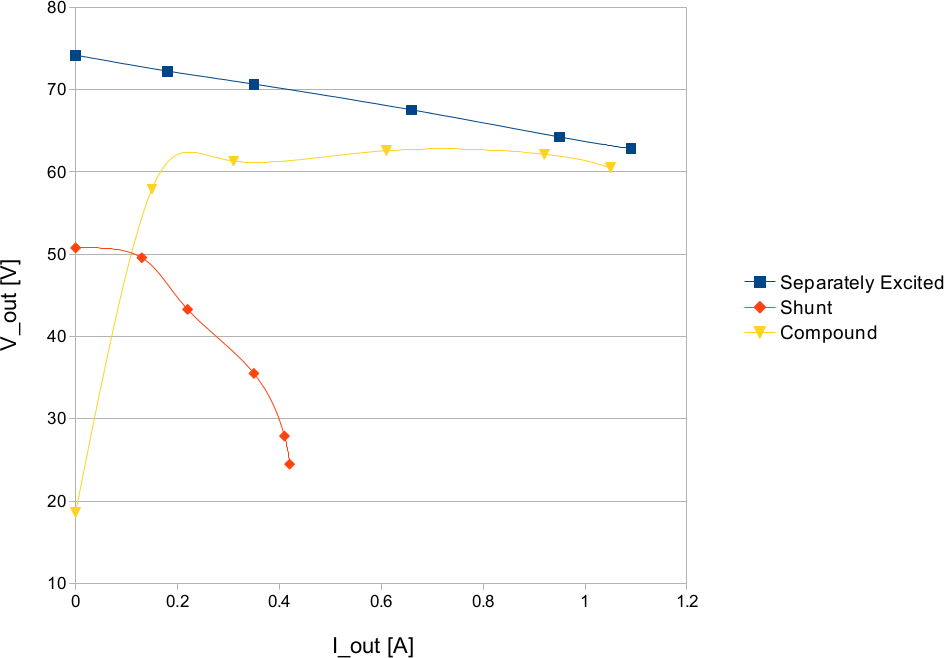
\includegraphics[width=0.8\textwidth]{img/graph}
    \caption{\textbf{Comparison}}
    \label{fig:graph}
\end{figure}

\section*{Conclusions}

For DC motors, the teminal characteristics are induced torque and motor speed. However, for DC generators the 
terminal characteristics are terminal voltage and line current, that is the output voltage and output current. 
In the figure above the terminal characteristics of a separately excited, shunt connected, and compound connected
DC generator are compared. In the plot of the terminal characteristics of a separately excited generator, it can 
be seen to be a straight line. As the load was increased in the experiment, the line current and thus the armature
current increased. From Kirchoff's voltage law $V_T = E_A - I_A*R_A$ the terminal voltage will thus decrease as
line current increases, and in a linearly fashion since the internal generated voltage $E_A$ is independent of the 
armature current $I_A$. The terminal characteristics of a shunt connected generator are similar to that of a 
separately excited generator. However, since the amount of field current depends of the terminal voltgae as the 
terminal voltage decreases then so does the field current. This causes the flux to decrease which then causes the 
internal genearated voltage $E_A$ to decrease and thus the terminal voltage decreases even more. 
\end{document}
